\documentclass{article}
\usepackage[utf8]{inputenc}
\usepackage[T1]{fontenc}
\usepackage[portuguese]{babel}
\usepackage{minted}
\usepackage{graphicx}
\graphicspath{{./images/}}

\title{Relatório RCOM T2}
\author{João Miguel, Miguel Barraca, Pedro Fernandes}
\date{Dezembro 2018}

\renewcommand*\contentsname{Sumário}

\begin{document}

\maketitle

\tableofcontents

\section{Introdução}
\section{Aplicação \textit{download}}
\subsection{Arquitetura}

A aplicação tem o objetivo de fazer o \textit{download} de um ficheiro recorrendo ao protocolo
FTP (\textit{File Transfer Protocol}). Para tal, recebe como argumento um link FTP, que deve conter
os seguintes campos:

\begin{itemize}
\item Nome de utilizador
\item Palavra-passe
\item Endereço do anfitrião
\item Caminho do ficheiro
\end{itemize}

Caso os dados do utilizador não sejam fornecidos, o programa pedi-los-á posteriormente.
Após a análise do argumento, o programa cria a ligação através de duas funções cujo código 
é já fornecido:

\begin{itemize}
\item \mintinline{C}{char *getServerIp(info_t info)}
\item \mintinline{C}{int createSocketTCP(char *server_ip, int server_port)}
\end{itemize}

Em caso de conexão bem sucedida, o programa segue os seguintes passos:
\begin{enumerate}
\item Enviar \mintinline{bash}{USER} e \mintinline{bash}{PASS}
\item Entrar em modo passivo \mintinline{bash}{pasv}
\item Criar novo socket TCP
\item Enviar comando \mintinline{bash}{RETR}
\item Transferir o ficheiro
\item Terminar a conexão com \mintinline{bash}{QUIT}
\end{enumerate}

Esta estrutura é apoiada nas seguintes funções, cuja documentação pode ser encontrada nos anexos:
\begin{itemize}
\item \mintinline{C}{int sendCommand(int socketFd, char *command, char *argument)}
\item \mintinline{C}{int readServerReply(int socketFd, char *reply)}
\item \mintinline{C}{void createFile(int fd, char *filename)}
\end{itemize}

E nas seguintes estruturas:

\begin{itemize}
\item \mintinline{C}{enum state_t}
\item[] Representa o estado da leitura da resposta aos comandos enviados.
\item \mintinline{C}{enum reply_type_t}
\item[] Representa o tipo da resposta do servidor aos comandos enviados. 
\item \mintinline{C}{struct info_t}
\item[] Guarda informação fornecida no argumento do programa. 
\end{itemize}


Ao longo do programa são impressas mensagens para informar o utilizador do avanço do processo.
\subsection{Exemplo de um \textit{download} com sucesso}
Após efetuar todas as experiências, o programa foi corrido com o argumento
ftp://ftp.up.pt/pub/sage/index.html.
O resultado é o que se pode observar nas imagens:
\begin{figure}[t]
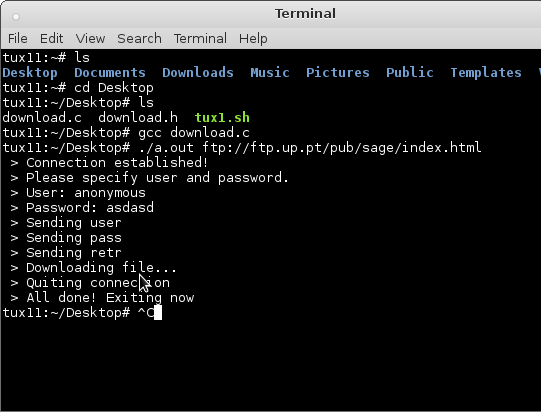
\includegraphics[width=8cm]{images/screen_dl.png}
\end{figure}

\begin{figure}[t]
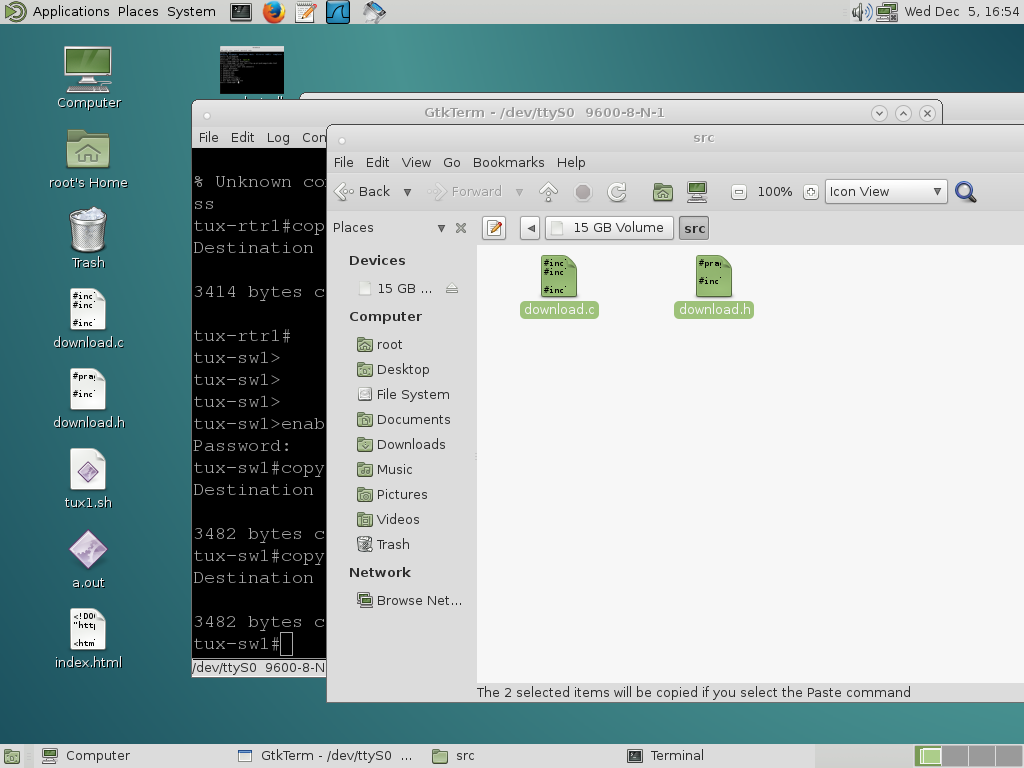
\includegraphics[width=8cm]{images/screen_dl_2.png}
\end{figure}

\begin{figure}
\end{figure}
\section{Configuração e análise de redes}
\subsection{Experiência 1 - Configurar uma rede IP}
\begin{enumerate}
\item O que são os pacotes ARP e para que são usados?

\item O que são os endereços MAC e IP dos pacotes ARP e porquê?

\item Que pacotes gera o comando \mintinline{bash}{ping}?

\item O que são os endereços MAC e IP dos pacotes \mintinline{bash}{ping}?

\item Como determinar se um quadro \textit{Ethernet} recebido é ARP, IP, ICMP?

\item Como determinar o tamanho de um quadro recebido?

\item Qual é a interface \textit{loopback} e porque é importante?
\end{enumerate}
\subsection{Experiência 2 - Implementar duas VLANs num \textit{switch}}
\begin{enumerate}
\item Como configurar a \textit{vlan10}?

\item Quantos domínios de transmissão existem? Como se pode concluir a partir dos registos?
\end{enumerate}
\subsection{Experiência 3 - Configurar um \textit{router} em Linux}
\begin{enumerate}
\item Que rotas existem nos \textit{tuxes}? Qual o seu significado?

\item Que informação contém uma entrada da tabela de encaminhamento?

\item Que mensagens ARP e endereços MAC associados são observados, e porquê?

\item Que pacotes ICMP são observados e porquê?

\item O que são os endereços IP e MAC associados aos pacotes ICMP e porquê?
\end{enumerate}
\subsection{Experiência 4 - Configurar um \textit{router} comercial e implementar NAT}
\begin{enumerate}
\item Como configurar uma rota estática num \textit{router} comercial?

\item Quais são os caminhos seguidos pelos pacotes nas experiências feitas e porquê?

\item Como configurar NAT num \textit{router} comercial?

\item O que faz NAT?
\end{enumerate}
\subsection{Experiência 5 - DNS}
\begin{enumerate}
\item Como configurar o servico DNS num anfitrião?

\item Que pacotes são trocados por DNS e que informação é transportada?
\end{enumerate}
\subsection{Experiência 6 - Conexões TCP}
\begin{enumerate}
\item Quantas conexões TCP são abertas pela aplicação FTP?

\item Em que conexão é transportada a informação de controlo FTP?

\item Quais são as fases de uma conexão FTP?

\item Como funciona o mecanismo ARQ TCP? Quais são os campos TCP relevantes? Que informação relevante pode ser observada nos
registos?

\item Como funciona o mecanismo de congestionamento de controlo TCP? Quais são os campos relevantes? Como é que
a taxa de transferência da conexão de dados evoluiu ao longo do tempo? Está de acordo com o mecanismo de congestionamento de controlo TCP?

\item A taxa de transferência de uma conexão de dados TCP é perturbada pelo aparecimento de uma segunda conexão TCP? Como?
\end{enumerate}
\section{Conclusão}
\section{Referências}
\section{Anexos}
\subsection{Código da aplicação \textit{download}}
\textbf{download.h}
\begin{minted}{c}
#pragma once

#include <stdbool.h>

#define MAX_BUF_SIZE 100
#define MAX_REPLY_SIZE 400
#define SOCKET_BUF_SIZE 1000
#define REPLY_CODE_SIZE 3
#define SERVER_PORT 21

typedef struct
{
    char serverName[MAX_BUF_SIZE];
    char filePath[MAX_BUF_SIZE];
    char fileName[MAX_BUF_SIZE];
    char user[MAX_BUF_SIZE];
    char pass[MAX_BUF_SIZE];
} info_t;

typedef enum
{
    READ_CODE,
    READ_LINE,
    READ_MULT_LINE,
    WAIT_FOR_PORT,
    FIRST_PORT_BYTE,
    SECOND_PORT_BYTE,
    END
} state_t;

typedef enum
{
    POSITIVE_PRE = 1,
    POSITIVE_INT,
    POSITIVE_COMP,
    TRANS_NEGATIVE_COMP,
    PERM_NEGATIVE_COMP
} reply_type_t;

/**
 * @brief Prints a message that shows how to run the program.
 * 
 * @param argv array of arguments passed from the command line
 * 
 * @return always return 1
 */
int usage(char *argv[]);

/**
 * @brief Parses the argument passed to the program, retrieving user information.
 * 
 * @param argument argument from the command line, supposedly an FTP link
 * @param info structure that holds user and server info
 * 
 * @return true if argument was successfully read, false otherwise 
 */
bool parseArgument(char *argument, info_t *info);

/**
 * @brief Gets a server ip from a host name
 * 
 * @param name host name
 * 
 * @return server ip 
 */
char *getServerIp(const char* name);

/**
 * @brief Creates a TCP socket, returning its respective file descriptor.
 * 
 * @param server_ip 
 * @param server_port 
 * 
 * @return socket's file descriptor 
 */
int createSocketTCP(char *server_ip, int server_port);

/**
 * @brief Reads the server reply to an FTP command, returning it through the reply argument.
 * 
 * @param socketFd socket's file descriptor
 * @param reply numeric descriptor of the server reply
 */
void readServerReply(int socketFd, char *reply);

/**
 * @brief Gets the server port after the program issues pasv command.
 * 
 * @param socketFd socket's file descriptor
 * 
 * @return the server port
 */
int getServerPort(int socketFd);

/**
 * @brief Sends and FTP command along with its argument (if applicable) and reads the server reply.
 * 
 * 
 * @param socketFd socket's file descriptor
 * @param command FTP command
 * @param argument command's argument, if any
 * 
 * @return 0 for POSITIVE_INT, 1 for POSITIVE_COMP and -1 for PERM_NEGATIVE_COMP
 */
int sendCommand(int socketFd, char *command, char *argument);

/**
 * @brief Called after sending RETR command, reads data from the socket and creates a local file.
 * 
 * @param fd second socket's file descriptor
 * @param filename name of the file to be retrieved
 */
void createFile(int fd, char *filename);
\end{minted}

\textbf{download.c}
\begin{minted}{C}
#include <arpa/inet.h>
#include <netinet/in.h>

#include <sys/socket.h>
#include <sys/types.h>

#include <ctype.h>
#include <errno.h>
#include <netdb.h>
#include <signal.h>
#include <stdio.h>
#include <stdlib.h>
#include <string.h>
#include <strings.h>
#include <unistd.h>
    
#include "download.h"

int usage(char *argv[])
{
    printf("Usage: %s ftp://[<user>:<password>@]<host>/<url-path>\n", argv[0]);
    return 1;
}

bool parseArgument(char *argument, info_t *info)
{
    char *sep;
    char* lastSep;
    int index1 = 6, index2;

    if (strncmp("ftp://", argument, 6) != 0)
        return false;

    if ((sep = strchr(argument + 6, ':')) != NULL)
    {
        int index;

        index = (int)(sep - argument);
        strncpy(info->user, argument + 6, index - 6);
        info->user[index - 6] = '\0';

        if ((sep = strchr(argument, '@')) == NULL)
            return false;

        int new_index = (int)(sep - argument);
        index++;
        strncpy(info->pass, argument + index, new_index - index);
        info->pass[new_index - index] = '\0';

        index1 = ++new_index;
    }
    else if ((sep = strchr(argument, '@')) != NULL)
        return false;
    else
        strncpy(info->user, "placeholder", 11);

    if ((sep = strchr(argument + 6, '/')) == NULL)
        return false;

    index2 = (int)(sep - argument);

    strncpy(info->serverName, argument + index1, index2 - index1);
    info->serverName[index2 - index1] = '\0';
    index2++;
    strncpy(info->filePath, argument + index2, strlen(argument) - index2);
    info->filePath[strlen(argument) - index2] = '\0';

    lastSep = strrchr(argument, '/');
    strcpy(info->fileName, lastSep + 1);
    info->fileName[strlen(lastSep)] = '\0';

    return true;
}

char *getServerIp(const char* name) 
{
    struct hostent *h;

    if ((h = gethostbyname(name)) == NULL) 
    {
        herror("gethostbyname");
        exit(1);
    }

    return inet_ntoa(*((struct in_addr *)h->h_addr_list[0]));
}

int createSocketTCP(char *server_ip, int server_port)
{
    int socketFd;
    struct sockaddr_in server_addr;

    /*server address handling*/
    bzero((char *)&server_addr, sizeof(server_addr));
    server_addr.sin_family = AF_INET;
    server_addr.sin_addr.s_addr =
        inet_addr(server_ip); /*32 bit Internet address network byte ordered*/
    server_addr.sin_port =
        htons(server_port); /*server TCP port must be network byte ordered */

    /*open an TCP socket*/
    if ((socketFd = socket(AF_INET, SOCK_STREAM, 0)) < 0)
    {
        perror("socket()");
        exit(0);
    }

    /*connect to the server*/
    if (connect(socketFd, (struct sockaddr *)&server_addr, sizeof(server_addr)) <
        0)
    {
        perror("connect()");
        exit(0);
    }

    return socketFd;
}

void readServerReply(int socketFd, char *reply)
{
    char c;
    int res = 0, i = 0;
    state_t state = READ_CODE;

    while (state != END)
    {
        if ((res = read(socketFd, &c, 1)) <= 0)
            continue;

        switch (state)
        {
        case READ_CODE:
            if (c == ' ')
            {
                state = READ_LINE;
                i = 0;
            }
            else if (c == '-')
            {
                state = READ_MULT_LINE;
                i = 0;
            }
            else if (isdigit(c))
            {
                reply[i++] = c;
            }
            break;
        case READ_LINE:
            if (c == '\n')
                state = END;
            break;
        case READ_MULT_LINE:
            if (c == reply[i])
            {
                i++;
            }
            else if (i == 3 && c == ' ')
            {
                state = READ_LINE;
            }
            break;
        case END:
            break;
        default:
            break;
        }
    }
}

int getServerPort(int socketFd)
{
    int res = 0;
    state_t state = WAIT_FOR_PORT;
    char c;
    char first_byte[4], second_byte[4];
    int numCommas = 0, i = 0;

    while (state != END)
    {
        if ((res = read(socketFd, &c, 1)) <= 0)
            continue;

        switch (state)
        {
        case READ_CODE:
            if (c == ' ')
            {
                if (i != 3)
                {
                    printf(" > Error receiving response code\n");
                    return -1;
                }
                i = 0;
                state = WAIT_FOR_PORT;
            }
            else
            {
                i++;
            }
            break;
            break;
        case WAIT_FOR_PORT:
            if (c == ',')
                numCommas++;

            if (numCommas == 4)
                state = FIRST_PORT_BYTE;
            break;
        case FIRST_PORT_BYTE:
            if (c == ',')
            {
                state = SECOND_PORT_BYTE;
                i = 0;
            }
            else
            {
                first_byte[i++] = c;
            }
            break;
        case SECOND_PORT_BYTE:
            if (c == ')')
                state = END;
            else
            {
                second_byte[i++] = c;
            }
            break;
        case END:
            break;
        default:
            break;
        }
    }

    return atoi(first_byte) * 256 + atoi(second_byte);
}

int sendCommand(int socketFd, char *command, char *argument)
{
    char reply[REPLY_CODE_SIZE];
    reply_type_t type;

    write(socketFd, command, strlen(command));
    if (argument != NULL)
        write(socketFd, argument, strlen(argument));
    write(socketFd, "\n", 1);

    while (true)
    {
        readServerReply(socketFd, reply);

        type = reply[0] - '0';

        switch (type)
        {
        case POSITIVE_PRE:
            break;
        case POSITIVE_INT:
            return 0;
        case POSITIVE_COMP:
            return 1;
        case TRANS_NEGATIVE_COMP:
            write(socketFd, command, strlen(command));
            if (argument != NULL)
                write(socketFd, argument, strlen(argument));
            write(socketFd, "\n", 1);
            break;
        case PERM_NEGATIVE_COMP:
            close(socketFd);
            return -1;
        default:
            break;
        }
    }
}

void createFile(int fd, char *filename)
{
    FILE *file = fopen(filename, "wb+");

    char fileData[SOCKET_BUF_SIZE];
    int nbytes;
    while ((nbytes = read(fd, fileData, SOCKET_BUF_SIZE)) > 0)
    {
        nbytes = fwrite(fileData, nbytes, 1, file);
    }

    fclose(file);
}

int main(int argc, char *argv[])
{
    info_t info;
    char *server_ip;
    char reply[MAX_REPLY_SIZE];
    int fd1, fd2, res, port;

    if (argc != 2 || !parseArgument(argv[1], &info))
        return usage(argv);

    server_ip = getServerIp(info.serverName);

    fd1 = createSocketTCP(server_ip, SERVER_PORT);
    readServerReply(fd1, reply);

    if (reply[0] == '2')
        printf(" > Connection established!\n");
    else
    {
        printf(" > Couldn't connect! Exiting.\n");
        exit(1);
    }

    if(strncmp(info.user, "placeholder", 11) == 0){
        printf(" > Please specify user and password.\n");
        printf(" > User: ");
        scanf("%s", info.user);
        printf(" > Password: ");
        scanf("%s", info.pass);
    }

    printf(" > Sending user\n");
    res = sendCommand(fd1, "user ", info.user);

    if (res == 0 || res == 1)
    {
        printf(" > Sending pass\n");
        res = sendCommand(fd1, "pass ", info.pass);
    }
    else
    {
        printf(" > Error sending username! Exiting.\n");
        exit(1);
    }

    write(fd1, "pasv\n", 5);
    port = getServerPort(fd1);

    fd2 = createSocketTCP(server_ip, port);

    printf(" > Sending retr\n");
    res = sendCommand(fd1, "retr ", info.filePath);

    if (res == 0)
    {
        printf(" > Downloading file...\n");
        createFile(fd2, info.fileName);
    }

    printf(" > Quiting connection\n");
    write(fd1, "quit\n", 5);

    close(fd1);
    close(fd2);

    printf(" > All done! Exiting now\n");
    return 0;
}    
\end{minted}
\subsection{Comandos de configuração}
De forma a facilitar a configuração dos \textit{tuxes}, foram desenvolvidos os seguintes \textit{bash scripts}.

\textbf{tux1.sh}
\begin{minted}{bash}
#!/bin/bash

if [ $# != 1 ] || [ $1 -lt 1 ] || [ $1 -gt 6 ]; then
    echo "Usage: $0 <stand>"
    exit 1
fi

ip1="172.16.$10.1/24"
ip2="172.16.$11.0/24"
ip3="172.16.$10.254"

ifconfig eth0 up
ifconfig eth0 $ip1
route add -net $ip2 gw $ip3
route add default gw $ip3
\end{minted}

\textbf{tux2.sh}
\begin{minted}{bash}
#!/bin/bash

if [ $# != 1 ] || [ $1 -lt 1 ] || [ $1 -gt 6 ]; then
    echo "Usage: $0 <stand>"
    exit 1
fi

ip1="172.16.$11.1/24"
ip2="172.16.$10.0/24"
ip3="172.16.$11.253"
ip4="172.16.$11.254"

ifconfig eth0 up
ifconfig eth0 $ip1
route add -net $ip2 gw $ip3
route add default gw $ip4
\end{minted}

\textbf{tux4.sh}
\begin{minted}{bash}
#!/bin/bash

if [ $# != 1 ] || [ $1 -lt 1 ] || [ $1 -gt 6 ]; then
    echo "Usage: $0 <stand>"
    exit 1
fi

ip1="172.16.$10.254/24"
ip2="172.16.$11.253/24"
ip3="172.16.$11.254"

ifconfig eth0 up
ifconfig eth0 $ip1
ifconfig eth1 up
ifconfig eth1 $ip2
echo 1 > /proc/sys/net/ipv4/ip_forward
echo 0 > /proc/sys/net/ipv4/icmp_echo_ignore_broadcasts
route add default gw $ip3
\end{minted}
\subsection{\textit{Logs} registados}

\end{document}
